\documentclass[11pt,a4paper]{report}
\usepackage[utf8]{inputenc}
\usepackage[italian]{babel}
\usepackage[pdftex]{hyperref}
\usepackage{tabularx}
\usepackage{graphicx}
\usepackage{epstopdf}
\usepackage{pdflscape}

\hypersetup{
	breaklinks,
	colorlinks,
	linkcolor=blue,
	pdftitle={Relazione},
	pdfsubject={Relazione sul progetto di Sistemi Concorrenti e Distribuiti},
	pdfauthor={Daniele Battaglia \& Davide Pesavento}
}

\title{Relazione sul progetto}
\author{Daniele Battaglia\\\url{dbat.fk@gmail.com}
	\and Davide Pesavento\\\url{davidepesa@gmail.com}}
\date{}

\newcommand{\term}[2]{\textbf{#1} & #2 \\}
\newcommand{\fun}[1]{\texttt{#1}}

\begin{document}

\maketitle

\tableofcontents

\clearpage

\chapter{Introduzione}
La presente relazione, assieme al software \textsl{FORSE}, è stata realizzata come prova d'esame per il corso "Sistemi Concorrenti e Distribuiti".

I requisiti considerati in fase di progettazione sono stati ricavati da quelli proposti dal docente (\url{http://www.math.unipd.it/~tullio/SCD/2008/Progetto.html})
secondo le clausole di partecipazione di livello 3.

\textsl{Formula One Race Simulation Engine} è realizzato utilizzando i linguaggi \textsl{Erlang} e \textsl{Python}. Per la distribuzione dell'applicazione abbiamo
usato il protocollo di distribuzione Erlang, supportato nativamente dall'omonimo linguaggio e implementato dalla libreria \textsl{Twotp} per il linguaggio
\textsl{Python}.
Per la creazione di interfacce grafiche è stata utilizzata la libreria \textsl{Qt4}.

Nelle fasi di progettazione e realizzazione del prototipo è stata posta maggiore attenzione riguardo le tematiche inerenti distribuzione e concorrenza, nozioni
centrali del corso, a scapito della parte riguardante la correttezza della simulazione da un punto di vista fisico. Abbiamo comunque cercato di includere
gli elementi essenziali della dinamica di una gara automobilistica anche se con alcune semplificazioni.

Nella prima parte del documento verranno esposti i requisiti espliciti, ricavati dalle richieste del docente, ed impliciti, estratti dal contesto reale che il software FORSE deve simulare.
Successivamente verranno elencati i problemi intrinseci che la progettazione del sistema deve affrontare e questi ultimi verranno analizzati alla luce delle conoscenze acquisite durante il corso.
Nella seconda parte della relazione verrà esposta la soluzione trovata, prima a livello progettual/architetturale, poi a livello di implementazione mostrando come i problemi precedentementi trovati vengano risolti in modo soddisfacente dal prototipo.


\chapter{Requisiti}
\begin{enumerate}
    \item Il sistema deve essere composto da più entità concorrenti e distribuite su una rete.
    \item La simulazione evolve in modo deterministico.
    \item Il circuito è suddiviso in settori ed è configurabile dall'utente tramite file di configurazione. Il file contiene le seguenti informazioni:
    \begin{itemize}
        \item[--] tipo di settore (rettilineo, curvilineo, entrata e uscita dai box, intermedio cronometrico, traguardo);
        \item[--] lunghezza e larghezza del segmento;
        \item[--] se il settore è una curva, direzione (destra o sinistra) e raggio di curvatura;
        \item[--] pendenza del suolo;
        \item[--] tempo atmosferico iniziale;
        \item[--] eventuali variazioni del tempo atmosferico nel corso della gara.
    \end{itemize}
    \item Insieme configurabile di concorrenti aventi le seguenti caratteristiche:
    \begin{itemize}
	\item[--] numero identificativo;
	\item[--] nome;
        \item[--] una scuderia di appartenenza;
        \item[--] esperienza/bravura;
        \item[--] peso;
        \item[--] vettura utilizzata.
    \end{itemize}
    \item Parametri di configurazione delle auto:
    \begin{itemize}
        \item[--] capienza del serbatoio;
	\item[--] quantità di carburante presente nel serbatoio a inizio gara;
        \item[--] tipo di pneumatici montato ad inizio gara (da asciutto, intermedio, da bagnato);
        \item[--] potenza del motore;
        \item[--] potenza dei freni;
        \item[--] peso a secco.
    \end{itemize}
    \item Parametri di configurazione di una competizione:
    \begin{itemize}
        \item[--] numero totale di giri da effettuare nella gara;
	\item[--] ordine di partenza dei piloti nella griglia di partenza;
    \end{itemize}
    \item Sistema di controllo (\textit{logging}):
    \begin{itemize}
        \item[--] un pannello generale con posizione dei concorrenti in gara, tempo attuale sul giro e tempo migliore sul giro;
        \item[--] situazione atmosferica della pista;
        \item[--] un pannello per ciascuna scuderia che riporta i parametri tecnici rilevanti delle vetture dei propri piloti (carburante residuo, usura dei pneumatici e loro tipo) nonché i tempi di percorrenza per settore di pista e totali.
    \end{itemize}
\end{enumerate}


%\chapter{\textit{Brainstorming}}
%Finora abbiamo preso in considerazione tre potenziali soluzioni.

%\section*{Soluzione 1}
%Vetture $\Rightarrow$ entità attive \\
%Segmenti del tracciato $\Rightarrow$ entità passive \\

%Per spostarsi da un segmento $S_1$ ad un altro segmento $S_2$ adiacente e successivo a $S_1$, una vettura deve assicurarsi che almeno una corsia di $S_2$ raggiungibile da $S_1$ sia libera, quindi dovrà già essere entrata nella regione protetta di una corsia di $S_2$. Il passaggio sarà completo quando la vettura esce dalla regione protetta di $S_1$ (e questo è un problema non banale). L'entità ``segmento'' espone solo un canale tipato. Le vetture dovranno fornire il numero della corsia da cui provengono e la logica che realizza i sorpassi è implementata nei segmenti effettuando una \texttt{requeue} presso la corsia appropriata.

%\section*{Soluzione 2}
%Segmenti del tracciato $\Rightarrow$ entità attive \\
%Vetture $\Rightarrow$ oggetti che vengono scambiati come parametri \\

%Ciascuna corsia di ciascun segmento è internamente suddivisa in tanti piccoli pezzi, ciascuno dei quali è dotato di una coda contenente le vetture in transito, ordinate per tempo di percorrenza crescente. L'entità ``segmento'' è in ascolto su un canale tipato asincrono, in attesa che il segmento precedente gli invii una nuova vettura. L'attesa prevede un \textit{timeout} pari al minimo tempo di percorrenza di tutte le vettura già accodate su ogni sottosegmento di ogni corsia. Non appena scade il \textit{timeout}, tutte le vetture con tempo di percorrenza pari al \textit{timeout} vengono fatte avanzare al sottosegmento successivo oppure inviate al segmento successivo. Come gestire canali e sorpassi? Usare un \textit{thread pool} per le vetture?

%\section*{Soluzione 3}
%Vetture $\Rightarrow$ entità attive \\
%Segmenti del tracciato $\Rightarrow$ entità passive \\

%Dopo aver calcolato il tempo di uscita della vettura dal segmento $S_i$, esso verrà immediatamente comunicato al segmento $S_{i+1}$ che lo inserirà in un'apposita struttura dati. I canali di ingresso in un settore hanno delle guardie che permettono l'accesso alle vetture solo nell'ordine prestabilito.


\chapter{Problemi}


\chapter{Architettura del sistema}
In questa sezione verranno descritte a livello funzionale le varie componenti del sistema e classificate secondo il modello visto a lezione.
\begin{landscape}
\begin{figure}
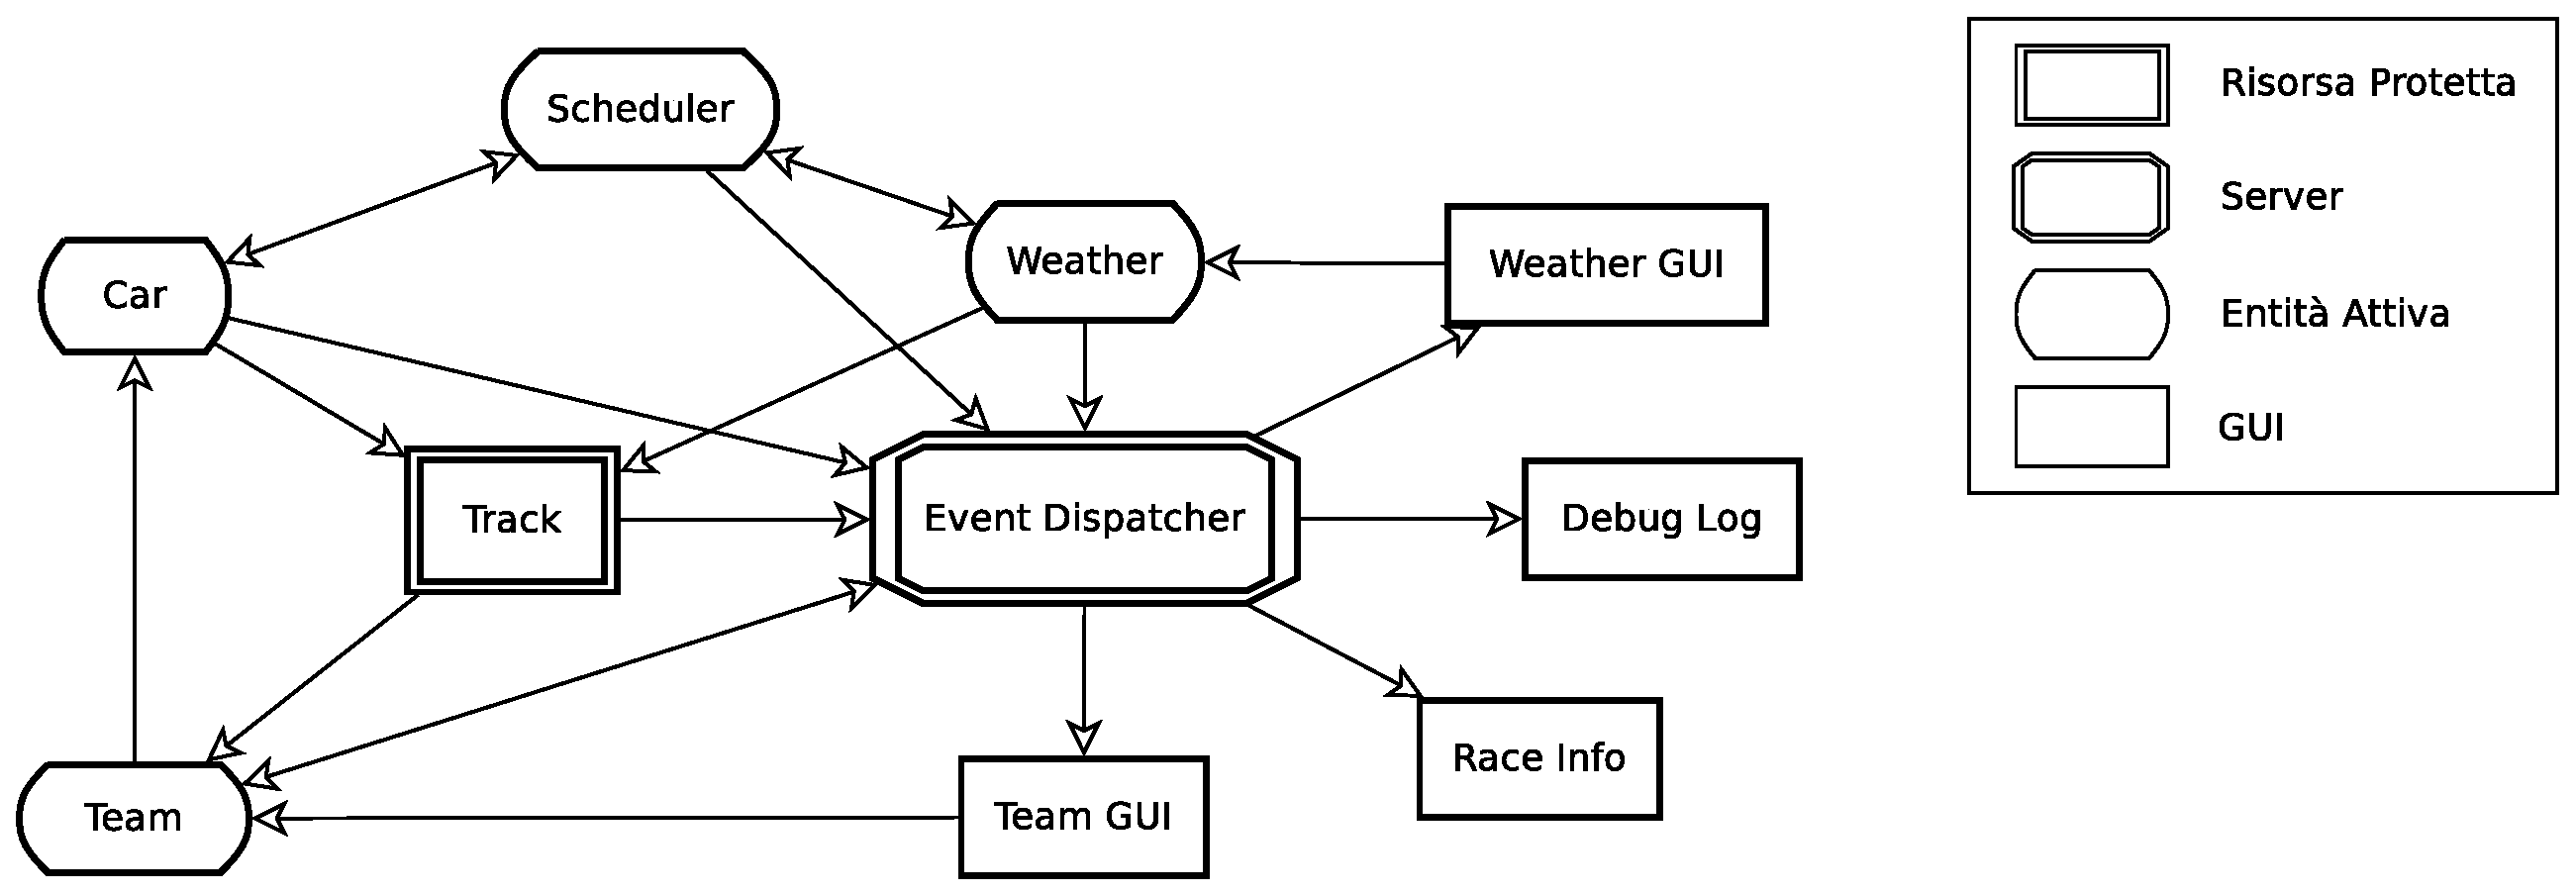
\includegraphics[height=.25\paperheight]{diagrammi/Arch}
\caption{Architettura di sistema}
\label{fig:architettura}
\end{figure}
\end{landscape}

\section{Scheduler}
La componente scheduler ha lo scopo di definire e gestire l'ordine con il quale i processi eseguono quando vanno a modificare i dati relativi alla componente track.
Tali processi possono essere per esempio i processi car che simulano gli spostamenti delle auto durante la gara oppure il processo che gestisce il tempo atmosferico
presente sulla pista.

L'idea di base di questa componente è di mantenere un orologio "logico" unico relativo alla competizione e di permettere l'esecuzione dei soli processi che si sono precendentemente prenotati per eseguire. Si tratta quindi di un sistema di booking nel quale i processi che vengono serviti devono prima indicare a che tempo relativo alla competizione vogliono eseguire e successivamente vengono messi in una coda ordinata secondo il tempo indicato nella prenotazione. Tra i vari processi presenti in questa coda lo scheduler eleggerà per l'esecuzione sempre quello in testa, ovvero il processo che nella fase di prenotazione precedente ha indicato un tempo minore.

Per poter soddisfare le caratteristiche sopra indicate è risultato naturale impostare l'entità scheduler come attiva.
Questa componente ha quindi la funzione di eliminare la parte indesiderata di concorrenza presente nel sistema, per rendere predicibile e controllata l'evoluzione del sistema.
\subsection*{Interfaccia Fornita}
Lo scheduler deve fornire un metodo \fun{queue\_work} che permette alle altre entità attive di effettuare la procedura di booking precedentemente descritta.
Il metodo \fun{set\_speedup} serve a regolare la velocità con cui evolve la simulazione, mentre i metodi \fun{start\_simulation} e \fun{pause\_simulation} servono rispettivamente ad avviare e fermare momentaneamente la simulazione.
\subsection*{Interfaccia Richiesta}
Nessuna.

\section{Track}
La componente track è stata pensata per incapsulare i dati relativi al circuito di gara e le regole di percorrenza del medesimo. Dal punto di vista progettuale track è sicuramente un'entità reattiva, in particolare una risorsa protetta con agente di controllo passivo.
I dati relativi alla configurazione della pista utilizzati dal sistema sono derivati dalle informazioni inserite dall'utente tramite file di configurazione.

La componente track deve contenere due gruppi di dati, uno riguardo le informazioni che possono essere considerate costanti poiché non variano nell'arco della competizione, l'altro comprendente i dati dinamici come la posizione delle vetture durante la gara.
La rappresentazione interna della pista è gestita come una lista di segmenti ciascuno dei quali contiene le seguenti informazioni:
\begin{itemize}
\item lunghezza del tratto,
\item ampiezza del segmento (espressa come numero di corsie),
\item inclinazione,
\item raggio di curvatura (nel caso in cui il segmento sia una curva).
\end{itemize}
Associate ai segmenti si hanno informazioni dinamiche riguardanti lo stato della pista come le condizioni atmosferiche al suolo (che può variare nel corso della competizione).
Un altro gruppo di informazioni dinamiche fondamentali contenute in track è quello relativo alle auto durante la competizione, per ogni auto infatti sono presenti:
\begin{itemize}
\item segmento che sta percorrendo,
\item tempo e corsia di ingresso,
\item tempo e corsia di uscita,
\item velocità di uscita.
\end{itemize}

Oltre ai dati visti finora, la componente track deve anche gestire la logica che determina quali spostamenti siano concessi alle auto e soprattutto secondo quali vincoli tali spostamenti siano possibili. Deve quindi esporre un metodo che permetta alle auto di simulare l'esito di un eventuale spostamento nella pista e un metodo che invece implementi l'effettivo spostamento dell'auto. Fornire un metodo per la simulazione della mossa permette di dare dei dati al chiamante che può quindi scegliere, secondo la sua logica interna e strategia di gara, quale sia la migliore mossa da eseguire e in un momento successivo effettuare tale mossa.
\subsection*{Interfaccia Fornita}
Grazie al metodo \fun{simulate} le entità car possono simulare, una volta scelta la corsia di uscita e espressa la "volontà" o meno di effettuare una sosta in quel giro, l'esito di uno spostamento.

L'utilità di questa funzionalità è evidente se si va a considerare il fatto che, essendo l'informazione ritornata dal metodo \fun{simulate} un'informazione basata sullo stato della pista e non su stime statiche, essa viene influenzata dalla posizione delle altre auto. Una scelta statica ragionevole del percorso migliore da seguire poterebbe essere quella individuata come traiettoria ottimale a circuito vuoto, tuttavia, in questo modo tutte auto seguirebbero lo stesso percorso non riuscendo mai a sorpassarsi.

Avendo a dispozione la posizione degli altri concorrenti è invece possibile per la componente car decidere di discostarsi dalla traiettoria ottimale cambiando corsia (operazione che aumenta il tempo di percorrenza del segmento) per effettuare manovre di sorpasso qualora sia possibile e vantaggioso.

Il metodo \fun{move} necessita degli stessi parametri del metodo \fun{simulate} e serve semplicemente a spostare effettivamente l'auto sul tracciato di gara e ad effettuare le eventuali notifiche di eventi scatenati da tale spostamento.
\subsection*{Interfaccia Richiesta}
Da un punto di vista funzionale la componente track contiene la logica che guida l'erogazione delle operazioni di rifornimento, tuttavia non può decidere quali operazioni effettuare, poiché questo tipo di scelte è inerente la strategia di gara e quindi è da considerarsi a carico della componente team. Di conseguenza track necessita di un metodo \fun{pitstop\_operations} da invocare presso la componente team associata all'auto ai box che abbia come valore di ritorno informazioni su che operazioni di rifornimento da effettuare.

Durante la simulazione, nel momento in cui un'auto effettua uno spostamento, è la componente track che riconosce eventi come un sorpasso o l'attraversamento di un intermedio cronometrico e deve provvedere ad inviare tali notifiche al sistema. La componente track non deve tuttavia incaricarsi di notificare direttamente tali eventi a chi interessato ma, come previsto dall'architettura di sistema, si limita ad inviare le notifiche alla componente event dispatcher e delega a quest'ultima la propagazione di tali informazioni nel sistema.
Le notifiche possibili riguardano:
\begin{itemize}
\item sosta ai box ed operazioni effettuate,
\item ritiro dalla gara di un'auto,
\item attraversamento di un intermedio cronometrico,
\item sorpasso,
\item fine della gara.
\end{itemize}

\section{Car}
Car è un'entità attiva e rappresenta nel contesto del progetto un'auto che partecipa alla competizione. Ad ogni istanza di questa componente presente nel sistema saranno associate queste informazioni:
\begin{itemize}
\item numero identificativo,
\item nome del pilota,
\item abilità del pilota,
\item peso del pilota,
\item scuderia di appartenenza,
\item livello di carburante nell'auto,
\item tipo di pneumatici utilizzati,
\item livello di usura dei pneumatici,
\item posizione nel circuito.
\end{itemize}
Prima dell'inizio della competizione car deve prenotarsi presso lo scheduler e stare poi in attesa del permesso di muoversi sulla pista dato dello scheduler.
Questa componente ha il compito di decidere quale traiettoria adottare per percorrere un segmento e deve farlo basandosi sullo stato dell'auto, sulle direttive dei team e dell'utente e sulle informazioni fornite da track.
\subsection*{Interfaccia Fornita}
L'autorizzazione a muoversi sul circuito di gara viene data a questa componente dallo scheduler attraverso l'invocazione del metodo \fun{move}. L'esecuzione di questo metodo è divisa in due fasi:
\begin{itemize}
\item simulazione, ovvero la fase in cui car utilizza l'interfaccia fornita dalla componente track per simulare tutte le mosse consentite e decidere, secondo la logica che governa la strategia di gara del pilota, quale tra le possibili traiettorie adottare.
\item spostamento, consiste nel segnalare a track la mossa deciso dall'auto e, a fronte delle conseguenze che tale spostamento comporta, prenotarsi nuovamente presso lo scheduler nel caso in cui la mossa vada a buon fine, ritirarsi altrimenti.
\end{itemize}

Per permettere la comunicazione della strategia di gara tra team e car, la presente componente deve esporre nella sua interfaccia un metodo \fun{set\_next\_pitstop} che serve alla scuderia per comunicare al pilota in quale giro recarsi ai box per il rifornimento.

L'utente può anche decidere di forzare il pilota ad effettuare mosse non previste dalla strategia di gara e che non possono essere modificate se non dall'utente stesso, in particolare può:
\begin{itemize}
\item imporre una sosta ai box il prima possibile, per questo viene fornito il metodo \fun{force\_pitstop},
\item forzare il ritiro dalla competizione di un'auto, a tale scopo viene esposto in interfaccia il metodo \fun{retire}.
\end{itemize}
\subsection*{Interfaccia Richiesta}
Questa componente necessita delle funzionalità \fun{simulate} (fase di simulazione) e \fun{move} (fase di spostamento) fornite dalla componente track per poter realizzare il metodo \fun{move} prima descritto.
Durante la fase di inizializzazione del sistema ogni componente car deve notificare i dati di interesse relativi alla sua configurazione al resto del sistema. Questo viene ottenuto grazie al canale \fun{notify} fornito dal event dispatcher.
\section{Team}
Questa componente nel contesto della simulazione rappresenta le scuderie in gara. Team deve quindi ricevere i dati relativi alle prestazioni delle proprie auto e allo stato della pista, elaborare una strategia di rifornimento e comunicare alle auto quando recarsi ai box.

Le decisioni che la logica di questa componente deve prendere sono inerenti le operazioni da eseguire in fase di rifornimento e comprendono la quantità di carburante aggiuntivo da imbarcare e se sostituire o meno i pneumatici ed eventualmente il tipo più appropriato alle condizioni atmosferiche della pista.
\subsection*{Interfaccia Fornita}
Team espone il metodo \fun{pitstop\_operations} nella sua interfaccia con lo scopo di fornire alla componente track, durante la fase di sosta ai box di un'auto, le informazioni necessarie ad effettuare le operazioni di rifornimento.

Il metodo \fun{update} serve a fornire un canale di comunicazione che l'event dispatcher usa per la notifica di eventi relativi alla gara considerati importanti per le scuderie.
\subsection*{Interfaccia Richiesta}
Per poter comunicare la strategia di gara decisa alle auto appartenenti alla scuderia rappresentata, questa componente necessita del metodo \fun{set\_next\_pitstop} fornito da car.
Come la componente car anche team deve comunicare le proprie informazioni di configurazione al sistema tramite il metodo \fun{notify} del event dispatcher.
\section{Event Dispatcher}
Questa componente ha il compito di ricevere tutti i dati relativi alla competizione e, dopo una eventuale rielaborazione, inviare tali dati alle componenti interessate.

Questo tipo di comunicazione segue il modello publish/subscribe ed è quindi previsto che le componenti del sistema interessate a tali dati effettuino prima la procedura di subscription (ricevendo se necessario lo stato attuale della competizione) per poi ottenere aggiornamenti con l'evolvere della gara. I subscribers devono indicare che informazioni desiderano ricevere di modo che l'event dispatcher possa effettuare una procedura di filtering per evitare l'invio di dati non necessari.

Viste le caratteristiche che deve avere tale componente, nell'ottica di un sistema distribuito, possiamo considerarla un server.
\subsection*{Interfaccia Fornita}
Il dispatcher deve fornire metodi di interfaccia verso due insiemi di attori:
\begin{itemize}
\item subscribers, ovvero i processi che si registrano per ottenere le informazioni riguardanti la gara attraverso il metodo \fun{subscribe},
\item notifiers, ovvero quei processi che scatenano eventi inerenti la competizione e delegano la notifica al sistema di tali eventi all'event dispatcher tramite l'invocazione del metodo \fun{notify}.
\end{itemize}
Il metodo \fun{subscribe} prevede che il processo chiamante indichi tra i parametri anche una funzione di callback che faccia da canale per l'invio delle notifche di gara.

\subsection*{Interfaccia Richiesta}
Da un punto di vista puramente pratico non vi è nessuna interfaccia richiesta da questa componente poiché il dispatcher, in assenza di observers, non effettua invocazioni di metodi. Tuttavia abbiamo preferito considerare l'interfaccia richiesta come dinamica, ovvero iniziamlemente vuota e che acquisisce metodi all'aumentare del numero di subscribers. Al momento della registrazione i subscribers devono indicare al dispatcher quale metodo di callback utilizzare e che va quindi ad aggiungersi all'interfaccia richiesta della presente componente.
\section{Weather}
Weather è la componente del sistema addetta a gestire le condizioni meteo iniziali sulla pista e le variazioni di tali condizioni durante la competizione. Le variazioni alla situazione meteo sono decise dall'utente tramite file di configurazione e possono essere decise a simulazione avviata in modo asincrono tramite interfaccia utente.

Poiché questa entità attiva va a modificare lo stato della pista, essa è evidentemente in concorrenza con le entità car presenti nel sistema. E' pertanto necessario che l'accesso alla risorsa track avvenga in modo controllato, in particolare è previsto che le modifiche sulla pista avvengano attraverso booking presso lo scheduler.
\subsection*{Interfaccia Fornita}
Al momento della prenotazione presso lo scheduler questa componente indica il metodo \fun{apply\_change} come metodo di callback, di conseguenza, nel momento in cui lo scheduler permetterà a questa entità di eseguire invocherà tale metodo. Questo metodo ha il compito di cambiare il tempo atmosferico di track secondo quanto definito dall'utente.
L'altro metodo che l'interfaccia di weather espone è \fun{schedule\_change} che serve per impostare eventuali variazioni nel tempo atmosferico da parte dell'utente a simulazione avviata.
\subsection*{Interfaccia Richiesta}
Conformemente a quanto visto finora anche la modifica del tempo atmosferico necessita dell'autorizzazione dello scheduler per essere portata a termine poiché modifica lo stato di track. Di conseguenza tutte le modifiche saranno procedute da un'invocazione del metodo \fun{queue\_work} dello scheduler per assolvere alla fase di prenotazione.

Le condizioni atmosferiche sono un fattore importante per la simulazione e una variazione delle medesime può essere di interesse a diverse componenti del sistema. Per questo motivo ogni volta che viene invocato il metodo \fun{apply\_change} viene notificata la modifica grazie al metodo \fun{notify} dell'event dispatcher.
\section{Debug Log}
Questa componente è pensata principalmente per essere d'ausilio nella fase di sviluppo e test. In fase di inizializzazione effettua la procedura di subscription presso l'event dispatcher per tutti i tipi di messaggi in modo da rendere i dati disponibili in formato testuale tramite una semplice interfaccia grafica.
\subsection*{Interfaccia Fornita}
Al fine di poter riceve le notifiche dall'event dispatcher questa componente espone in interfaccia un metodo callback che serve a ricevere le notifiche e mostrare le informazioni trasportate in forma testuale all'utente.
\subsection*{Interfaccia Richiesta}
Facendo parte del gruppo di componenti observers, debug log necessita della possibilità di registrarsi presso l'event dispatcher con il metodo \fun{subscribe}.
\section{Race Info}
Questa componente serve a raggruppare la maggior parte delle funzionalità di visualizzazione della competizione e permette inoltre all'utente di interagire con il sistema.

I dati visualizzati devono essere sufficienti all'utente per comprendere l'andamento della gara. Devono quindi essere presenti:
\begin{itemize}
\item stato della simulazione (avviata, in pausa, terminata),
\item posizione delle auto sulla pista,
\item classifica e sorpassi,
\item eventuali ritiri,
\item velocità massima,
\item tempo migliore sul giro.
\end{itemize}
Attraverso questa componente l'utente può interagire con lo stato della simulazione nei seguenti modi:
\begin{itemize}
\item avvio,
\item pausa,
\item terminazione,
\item cambio del fattore di speedup.
\end{itemize}
\subsection*{Interfaccia Fornita}
Essendo race info una GUI dal punto di vista funzionale espone sicuramente un'interfaccia verso l'utente con lo scopo di rendere facilmente fruibili i dati riguardanti l'evolvere della simulazione.
Questa componente, conformemente a quanto avviene nel resto del sistema, riceve le informazioni sulla competizione dall'event dispatcher. Per questo motivo deve fornire al dispatcher almeno un canale di comunicazione (metodo di callback).
\subsection*{Interfaccia Richiesta}
Per poter interagire con la simulazione come descritto precendentemente race info necessita di diversi metodi forniti della componente scheduler:
\begin{itemize}
\item \fun{start\_simulation},
\item \fun{pause\_simulation},
\item \fun{set\_speedup}.
\end{itemize}
Appartenendo inoltre al gruppo degli observers questa componente necessita del metodo del event dispatcher \fun{subscribe}.
\section{Team Gui}
Questa componente è un'interfaccia grafica che serve a fornire all'utente dettagli approfonditi sulle statistiche di gara delle auto appartenenti ad una scuderia.
I dati da mostrare all'utente sono:
\begin{itemize}
\item nome del pilota,
\item carburante residuo,
\item consumo medio di carburante sull'ultimo giro,
\item tipo e stato dei pneumatici,
\item usura media dei pneumatici sull'ultimo giro,
\item tempo migliore per intermedio cronometrico,
\item tempo migliore sul giro,
\item numero di pitstop effettuati,
\item operazioni effettuate durante l'ultima sosta ai box.
\end{itemize}
L'utente può inoltre forzare la sosta ai box o il ritiro per un'auto appartenente alla scuderia.
\subsection*{Interfaccia Fornita}
\subsection*{Interfaccia Richiesta}
\section{Weather Gui}
Questa componente è un'interfaccia grafica che mostra all'utente le condizioni atmosferiche sulla pista e permette a quest'ultimo di modificarle in modo asincrono rispetto alla simulazione durante il corso della competizione. Le informazioni sullo stato della pista sono ottenute dall'event dispatcher mentre le richieste di variazioni vengono inviate alla componente weather.

\subsection*{Interfaccia Fornita}
\subsection*{Interfaccia Richiesta}
\section{Avvio e Terminazione}
Infrastruttura e meccanismi di avvio e terminazione del sistema.
\section{Alternative?}
Eventualmente cassare questa sezione

\chapter{Implementazione}
\section{Tecnologie utilizzate}
Breve descizioni dei principi base ed eventuali problemi riscontrati.
\section{Dinamiche della competizione}
\subsection{Partenza}
Prima che l'utente dia il via alla competizione tutte le auto devono essersi registrate presso lo scheduler indicando come tempo di prenotazione 0.
E' importante precisare che in questa situazione l'ordine in cui lo scheduler fa eseguire i processi car non influenza l'esito della gara infatti alla partenza le auto sono tutte su segmenti diversi e di conseguenza non conocorrono tra di loro per l'accesso ad uno stesso segmento. Ne deriva quindi che sebbene l'ordine di esecuzione alla partenza possa essere considerato casuale (dipende dall'ordine di registrazione presso una componente distribuita del sistema), questo non va ad influenzare i tempi di percorrenza dei segmenti da parte delle auto e non influisce quindi con il risultato della gara.
La disposizione iniziale delle auto sulla pista avviene similmente a quanto riportato in figura \ref{fig:startGrid}, ed è richiesto all'utente che nella zona di pista che precede la linea di arrivo vi siamo almeno tre corsie.
\begin{figure}[h]
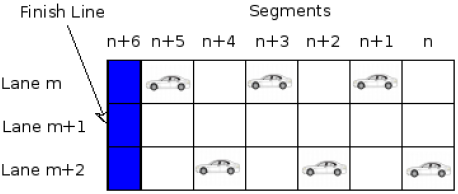
\includegraphics[scale=0.7]{diagrammi/StartGrid}
\caption{Griglia di Partenza}
\label{fig:startGrid}
\end{figure}
\subsection{Percorrenza di un Segmento}
Descrizione dell'algoritmo
\subsection{Intermedi Cronometrici}
\subsection{Pit Lane}
Descrizione dell'implementazione delle regole di accesso ai box, struttura della pista e algoritmo di sosta e rifornimento dell'auto.
\subsection{Arrivo}
Termiazione dei processi car
\subsection{Interazione con l'Utente}

\section{Correttezza}
Considerazioni sulla correttezza del tempo di percorrenza, controllo della concorrenza, algoritmo di sorpasso.
Rallentamento della simulazione non influenza i tempi di gara (scheduler).
\appendix

\chapter{Glossario}

\begin{tabularx}{\textwidth}{lX}
\term{Intermedio cronometrico}{}
\term{Segmento}{L'unità di spazio più piccola e indivisibile che costituisce il tracciato, utilizzata per la rappresentazione interna dello stesso.}
\term{Settore}{Porzione di tracciato che presenta caratteristiche fisiche costanti per tutta la sua lunghezza. Definito dall'utente in fase di configurazione.}
\term{Speedup}{Fattore numerico che serve ad impostare la velocità con la quale la simulazione evolve.}
\end{tabularx}

\end{document}
